% !TEX encoding=utf8
\documentclass[10pt,a4paper]{scrartcl}

\usepackage{ucs}
\usepackage[utf8]{inputenc}
\usepackage[ngerman]{babel}
\usepackage{amsmath}
\usepackage{amssymb, amstext}
\usepackage{mathtools}
\usepackage[pdftex]{graphicx}
\usepackage{bibgerm}
\usepackage{amsthm}
\usepackage[colorlinks=true]{hyperref}
\usepackage{dsfont}
\usepackage{caption}
\usepackage{multicol}
\usepackage{pdfpages}
\usepackage{listings}
\usepackage[a4paper,left=2.5cm,right=2.5cm,top=2cm,bottom=4cm,bindingoffset=5mm]{geometry}
\usepackage{tikz}
%\usepackage{txfonts}
\usepackage{textcomp}
\usepackage{multirow}
\pagestyle{headings}
\usepackage{tabularx}
\usepackage{enumerate}
\newcolumntype{L}[1]{>{\raggedright\arraybackslash}p{#1}} % linksbündig mit Breitenangabe
\newcolumntype{C}[1]{>{\centering\arraybackslash}p{#1}} % zentriert mit Breitenangabe
\newcolumntype{R}[1]{>{\raggedleft\arraybackslash}p{#1}} % rechtsbündig mit Breitenangabe
\usepackage{subfig}

\setlength{\topmargin}{-15mm}
%\setcounter{secnumdepth}{5} %wie viele Level


%\usepackage[latin1]{inputenc}
\usepackage[T1]{fontenc}
%\usepackage{ae,aecompl}
%\usepackage{amsmath,amssymb,amstext}
\usepackage{psfrag}
\usepackage{caption}
\usepackage{booktabs}
\usepackage{tabularx}
\captionsetup[table]{textfont=it,justification=raggedright,singlelinecheck = false}
\usepackage{float}




%%%%

% einige Abkuerzungen
\newcommand{\C}{\mathbb{C}} % komplexe
\newcommand{\K}{\mathbb{K}} % komplexe
\newcommand{\R}{\mathbb{R}} % reelle
\newcommand{\Q}{\mathbb{Q}} % rationale
\newcommand{\Z}{\mathbb{Z}} % ganze
\newcommand{\N}{\mathbb{N}} % natuerliche

%Zum markieren: http://texwelt.de/wissen/fragen/2803/wie-kann-ich-formel-teile-einer-gleichung-einkreisen
\newcommand\mrahmen[3][]{%
  \tikz[anchor=base,baseline]\node[inner sep=2pt,draw=#2,#1]{$\displaystyle#3\mathstrut$};}
\colorlet{mfarbe}{red}


%verschiednen sachen die man mit begin{...} dann einzeln durchnummerrienen lassen kann
\newtheorem{defin}{Definition}
\newtheorem{satz}{Satz}
\newtheorem{formel}{Formel}
\newtheorem{abbildung}{Abbildung}
\newtheorem{versuch}{Versuch}


%Titel Gedöns
\title{Versuch F09\\ Neuromorphic Computing}
\date{Lab book}
\author{Xeno Boecker, Jan Jakob}
\date{}

\begin{document}


\pagenumbering{roman} %% small roman page numbers

%%% include the title
\thispagestyle{empty}  %% no header/footer (only) on this page
 \maketitle

%%% start a new page and display the table of contents
\newpage
\tableofcontents

%%% start a new page and display the list of figures
%\newpage
%\listoffigures

%%% start a new page and display the list of tables
%\newpage
%\listoftables

%%% display the main document on a new page 
\newpage

\pagenumbering{arabic} %% normal page numbers (include it, if roman was used above)


\section{Untersuchung eines einzelnen Neurons}

Im ersten Experiment untersuchen wir das Zündverhalten eines einzelnen Neurons ohne Input / äußere Stimuli. Das Neuron kann in einen kontinuierlichen Feuerzustand versetzt werden, wenn das Leck-Umkehrpotential die Zündschwelle übersteigt.

\subsection{Aufgabe 1}
Im Folgenden zeichnen wir ein Ersatzschaltbild eines Neurons in der beschriebenen Konfiguration. Dazu nehmen wir das Neuronenschema in Abbildung 5 als Referenz und stellen uns das Neuron als einen Kondensator vor, der an mehrere Spannungsquellen angeschlossen ist. Die verschiedenen Ionenkanäle der Nervenzelle werden zu einem
einem einzigen erregenden und einem einzigen hemmenden Potenzial zusammengefasst, und die Diffusion durch die Membran wird durch das Leckpotential ersetzt.

\begin{figure} [ht]
\begin{center}
\includegraphics[scale=0.5]{pictures/Neuron_Circuit.png}
\caption{Ersatzschaltbild eines Neurons in der beschriebenen Konfigurationn}
\label{fig:schaltung1}
\end{center}
\end{figure}

\noindent \textbf{Frage:} Welche Parameter des Neurons beeinflussen die Feuerrate?

\begin{enumerate}
\item Refraktärzeit $\tau_{refrac}$
\item Membranzeitkonstante $\tau_m=\frac{C_m}{gl}$ 
\item Schwellwert- und Resetspannung $V_{th} , V_{reset}$
\end{enumerate}


\subsection{Aufgabe 2}
Bei dieser Aufgabe haben wir nur wie in der Versuchanleitung beschrieben Vorbereitungen getroffen und die aktuelle Shell für die Verwendung von Spikey eingerichtet.


\subsection{Aufgabe 3}
\noindent Auf dem Spikey-Chip wird ein einzelnes Neuron mit folgenden Parametern konfiguriert:

\begin{table}[H]
\centering
\captionsetup{justification=centering}
\caption{Parameter für ein einzelnes Neuron}
\begin{tabular}{l|l}
 Parameter&Wert\\
\hline
$V_{reset}$&$-80.0$mV\\
$E_{rev_I}$&$-75.0$mV\\
$V_{rest}$&$-50.0$mV\\
$V_{thresh}$&$-55.0$mV\\
$g_{leak}$&$20.0$
\end{tabular}
\label{tab:01}
\end{table}

\noindent Der Potentialverlauf ist in Abbildung \ref{fig:abb2} dargestellt. Wir lesen für die Werte $V_{reset}$ und $V_{th}$ folgende Werte ab:

\begin{table}[H]
\centering
\captionsetup{justification=centering}
\caption{Abgelesene Werte aus dem Verlauf des Membranpotentials}
\begin{tabular}{l|l}
 Parameter&Wert\\
\hline
$V_{reset}$&$-83.0 \pm 3.0$mV\\
$V_{thresh}$&$-56.0 \pm 3.0$mV
\end{tabular}
\label{tab:02}
\end{table}

\noindent Die Werte liegen jeweils im $3\sigma$-Bereich.
\begin{figure} [ht]
\begin{center}
\label{fig:abb2}
\caption{Verlauf des Membranpotentials}
\includegraphics[scale=0.5]{experiments/SingleNeuron/fp_task1_1membrane.png} 
\end{center}
\end{figure}


\subsection{Aufgabe 4}
Durch Einsatz des Oszilloskops bestimmen wir die durchschnittliche Feuerrate des Neurons und ihre Standardabweichung mit Hilfe der Mess- und Statistikfunktion. Wir erhalten folgende Ergebnisse: 

\begin{align*}
f_{firing} = 355.4 \pm 3.4 kHz
\end{align*}

\begin{figure} [ht]
\begin{center}
\label{fig:abb3}
\caption{durchschnittliche Feuerrate durch Einsatz des Oszilloskops}
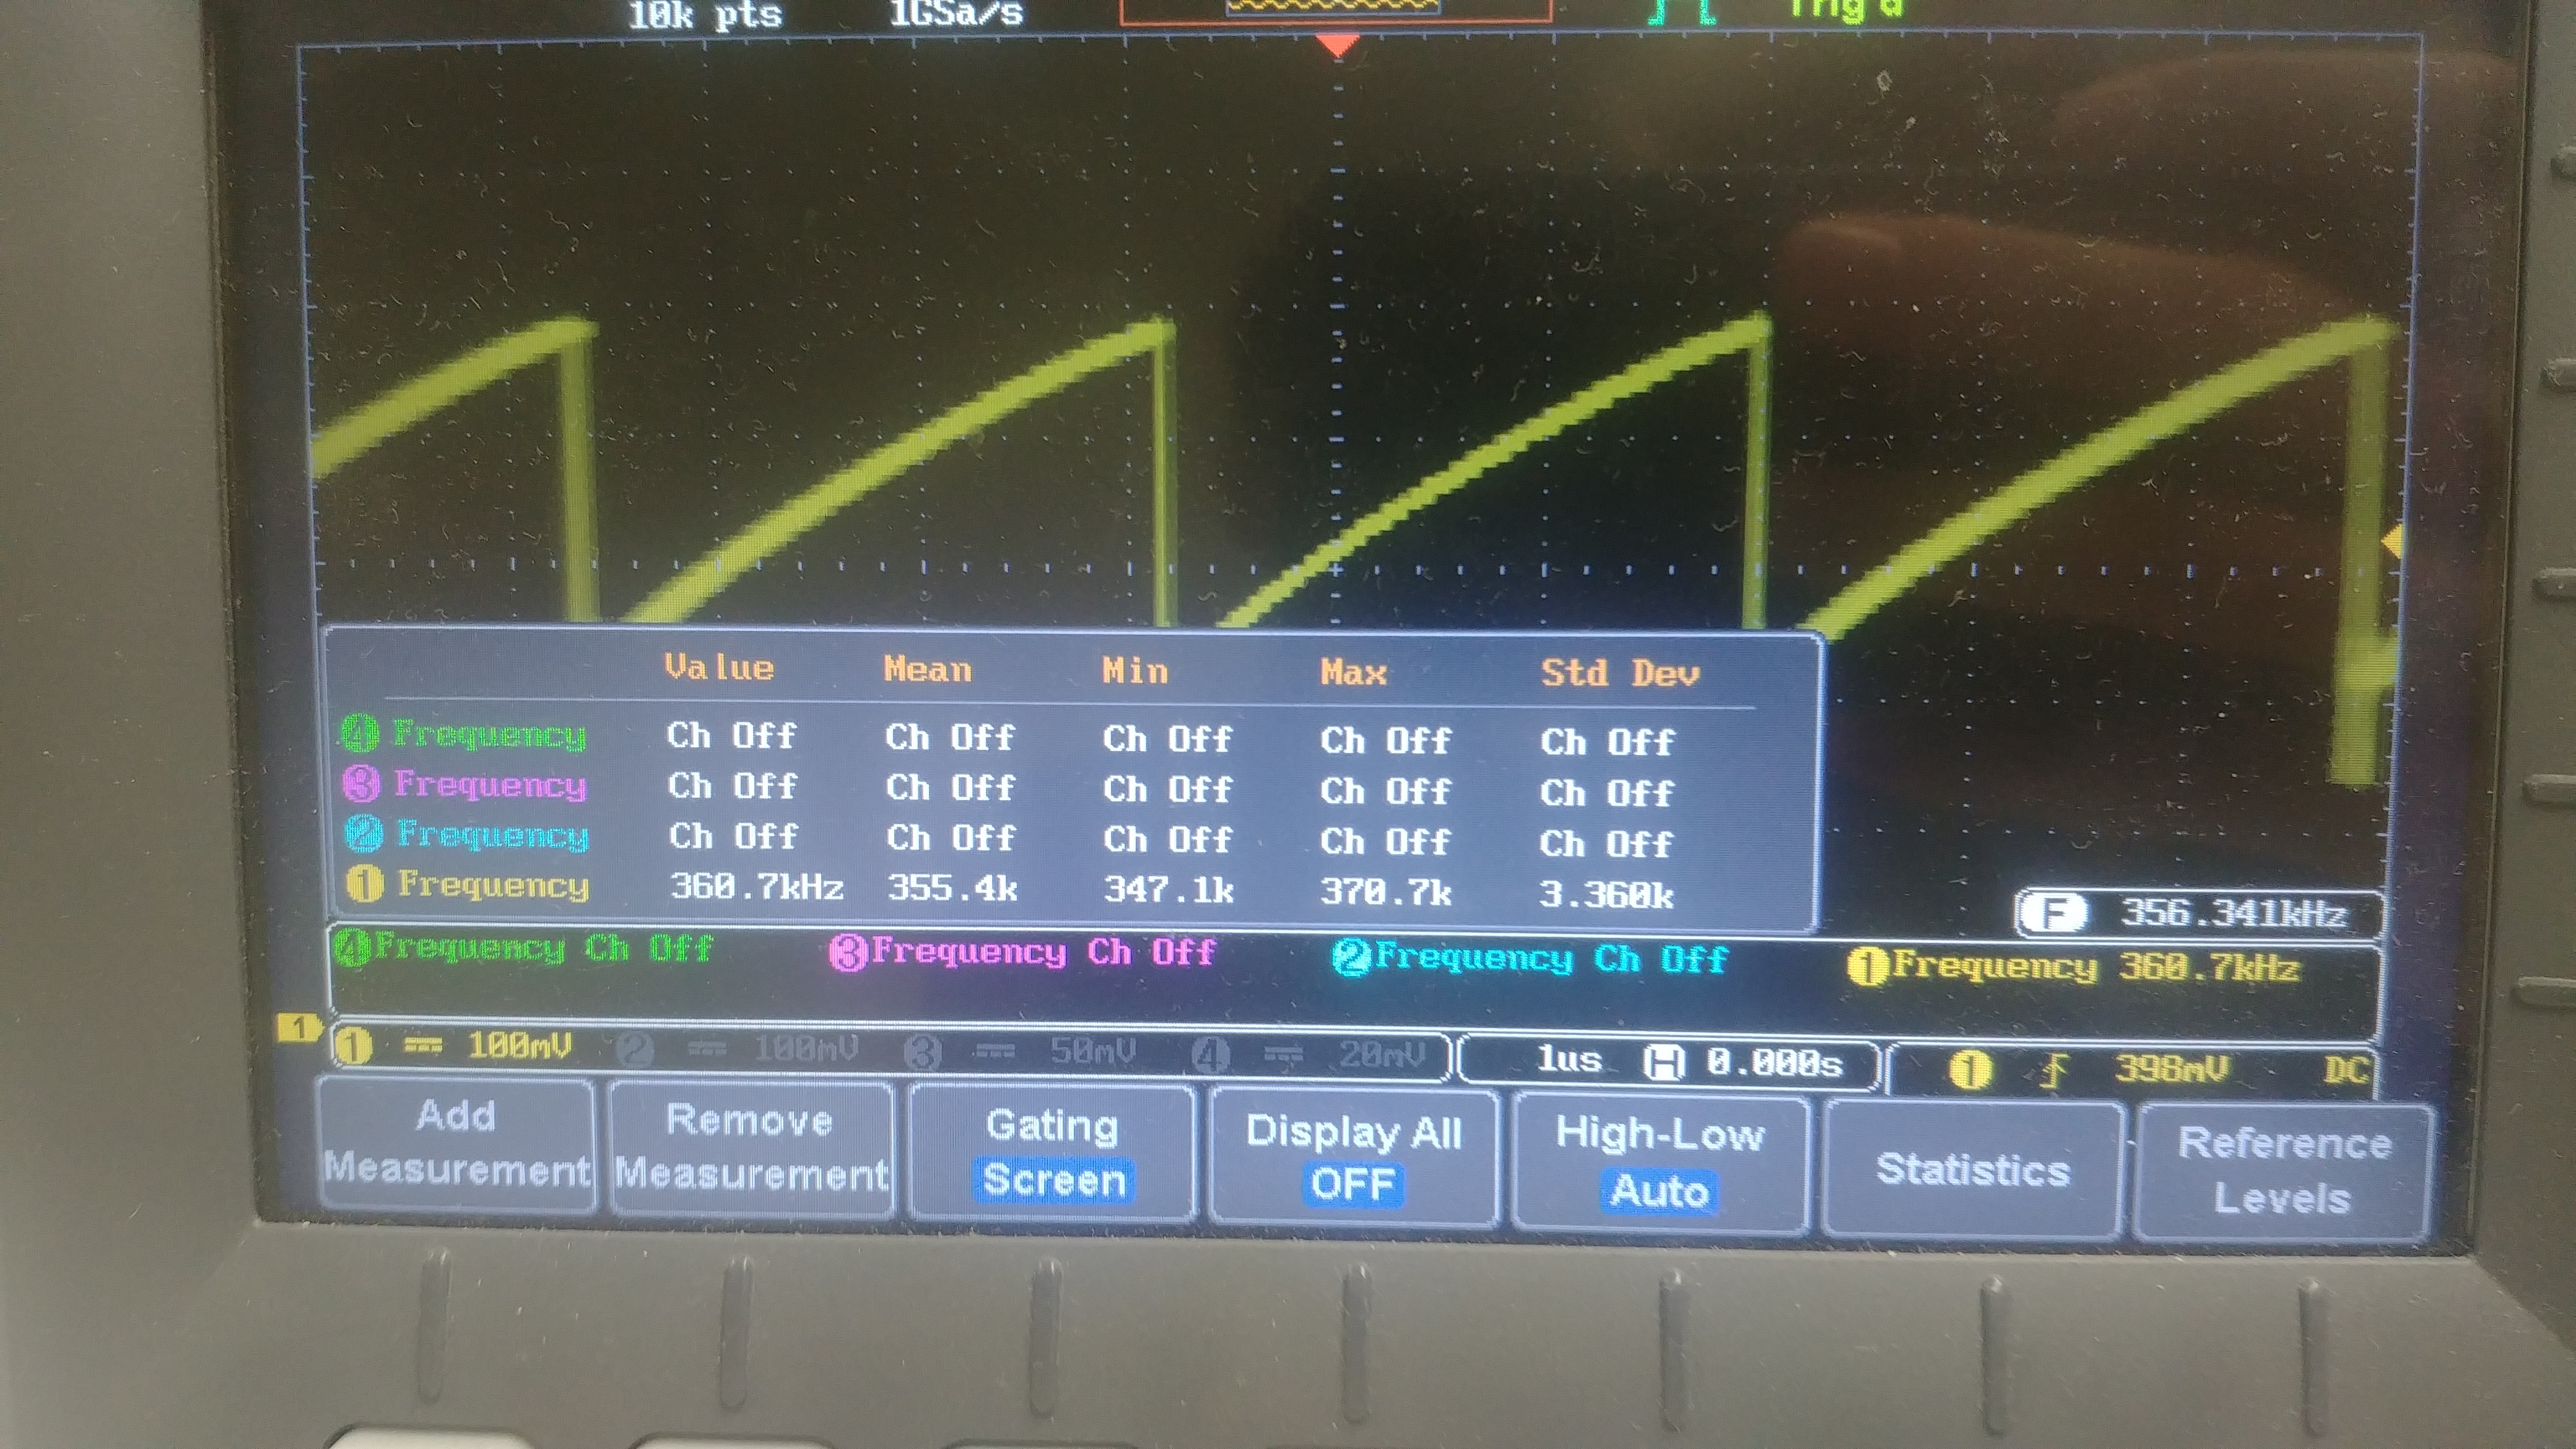
\includegraphics[scale=0.06]{pictures/oszilloskop_pic_1.jpg} 
\end{center}
\end{figure}

\noindent Wir berechnen die mittlere Feuerrate der im Spikes-Array empfangenen Spikes und vergleichen sie mit der Messung des Oszilloskops. Um eine Verteilung der Interspike-Intervalle (ISI) zu erhalten, berechnen wir die paarweise Differenz der empfangenen Spike-Zeiten und speichern sie in einem neuen Array. Den
Mittelwert dieser Differenzen und seine Standardabweichung berechnen wir mit den
entsprechenden NumPy-Funktionen.

\lstset{language=Python}
\lstset{frame=lines}
\lstset{caption={Berechnung der mittleren Feuerrate}}
\lstset{label={lst:code_direct}}
\lstset{basicstyle=\footnotesize}
\begin{lstlisting}
# time differences
timeDifferences = np.diff(spikes)

print("time differences mean", np.mean(timeDifferences))
print("time differences std deviation", np.std(timeDifferences))

print("firing rate mean", 1e4 / np.mean(timeDifferences))
print("firing rate std deviation", 1e4 / np.std(timeDifferences))
\end{lstlisting}
%\lstinputlisting[language=Python]{mesh.py}

\noindent Damit erhalten wir in Übereinstimmtung mit der obig bestimmten Feuerrate einen Wert von

\begin{align*}
f_{firing} = 356.5 \pm 4.7kHz.
\end{align*}

\noindent Den Faktor $1e4$ benötigen wir zur Umrechnung von biologischen Zeitskalen auf Chip-Zeitskalen.

\newpage


\section{Kalibrierung der Neuron-Parameter}
Durch Produktionsschwankungen bei der Herstellung des Chips kommt es zur sogenannten fixed pattern noise, was dazu führt, dass die Neuronen und die Synapsen-Parameter über den Chip variieren. Dies lässt sich durch Kalibrationsroutinen minimieren, was hier am Beispiel der Membranzeitkonstante $\tau_m$ durchgeführt wird. 

\subsection{Aufgabe 1}
Zunächst berechnen wir die theoretische Feuerrate aus den voreingestellten Werten. Nach Gleichung (6) aus der Versuchsanleitung gilt:
\begin{equation}
I_m(t)=C_m\frac{dV_m(t)}{dt}=g_l(E_l- V_m(t))
\end{equation} 
Nach Lösen der DGL erhält man:
\begin{equation}
V_m(t)=E_{leak} + (V_{res}-E_{leak})\cdot e^{-\frac{1}{\tau_m t}}
\end{equation}
Es soll nun 
\begin{equation}
V_m(t)=V_{thresh}
\end{equation}
gelten. Mit den Werten aus dem Pythonskript erhält man nach Umformen von (3) nach t einen Wert von:
\begin{equation*}
f_{firing}=-52.86 Hz
\end{equation*}
Die dabei verwendeten Werte für $V_{thresh}$ usw. entsprechen den in Versuchsteil 1 verwendeten Werten und können Tabelle 1 entnommen werden.


\subsection{Aufgabe 2}
Wir setzen den Schwellwert gerade auf den 1/e-ten Teil über $V_{reset}$, damit ist dieser nach $\tau_m$ erreicht. Eine Periode hat also gerade die Dauer $\tau_m + \tau_{refrac}$.
\begin{equation}
V_m(t = 1 / \tau_m) = V_{thresh} = E_{leak} + (V_{res}-E_{leak})\cdot e
\end{equation}
Stellen wir Gleichung (4) nach $V_{thresh}$, so erhalten wir
\begin{equation}
V_{thresh} = E_{leak} - 1/e\cdot (E_{leak} - V_{reset}),
\end{equation}
in Übereinstimmung mit Gleichung (8) aus der Versuchsanleitung. Mit den Parametern aus dem Skript ergibt sich ein neuer Wert von 
\begin{equation}
V_{thresh}=-51.69mV.
\end{equation}


\subsection{Aufgabe 3}
Wir ändern die Einstellung für $V_{thresh}$ im Skript entsprechend und führen das Skript aus. Außerdem stellen wir die Oszilloskop-Aufzeichnung so ein, dass alle 4 Membranspannungen zu sehen sind (Abbildung \ref{fig:abb4}). Wir verwenden die Messfunktionen des Oszilloskops, um gleichzeitig die Feuerfrequenz der vier angeschlossenen Neuronen zu messen. Außerdem aktivieren wir die Statistikfunktion, damit das Oszilloskop Mittelwerte und Standardabweichung berechnet. Wir erhalten folgende Werte:

\begin{figure} [ht]
\begin{center}
\label{fig:abb4}
\caption{Membranspannungen bei vier verschiedenen Neuronen}
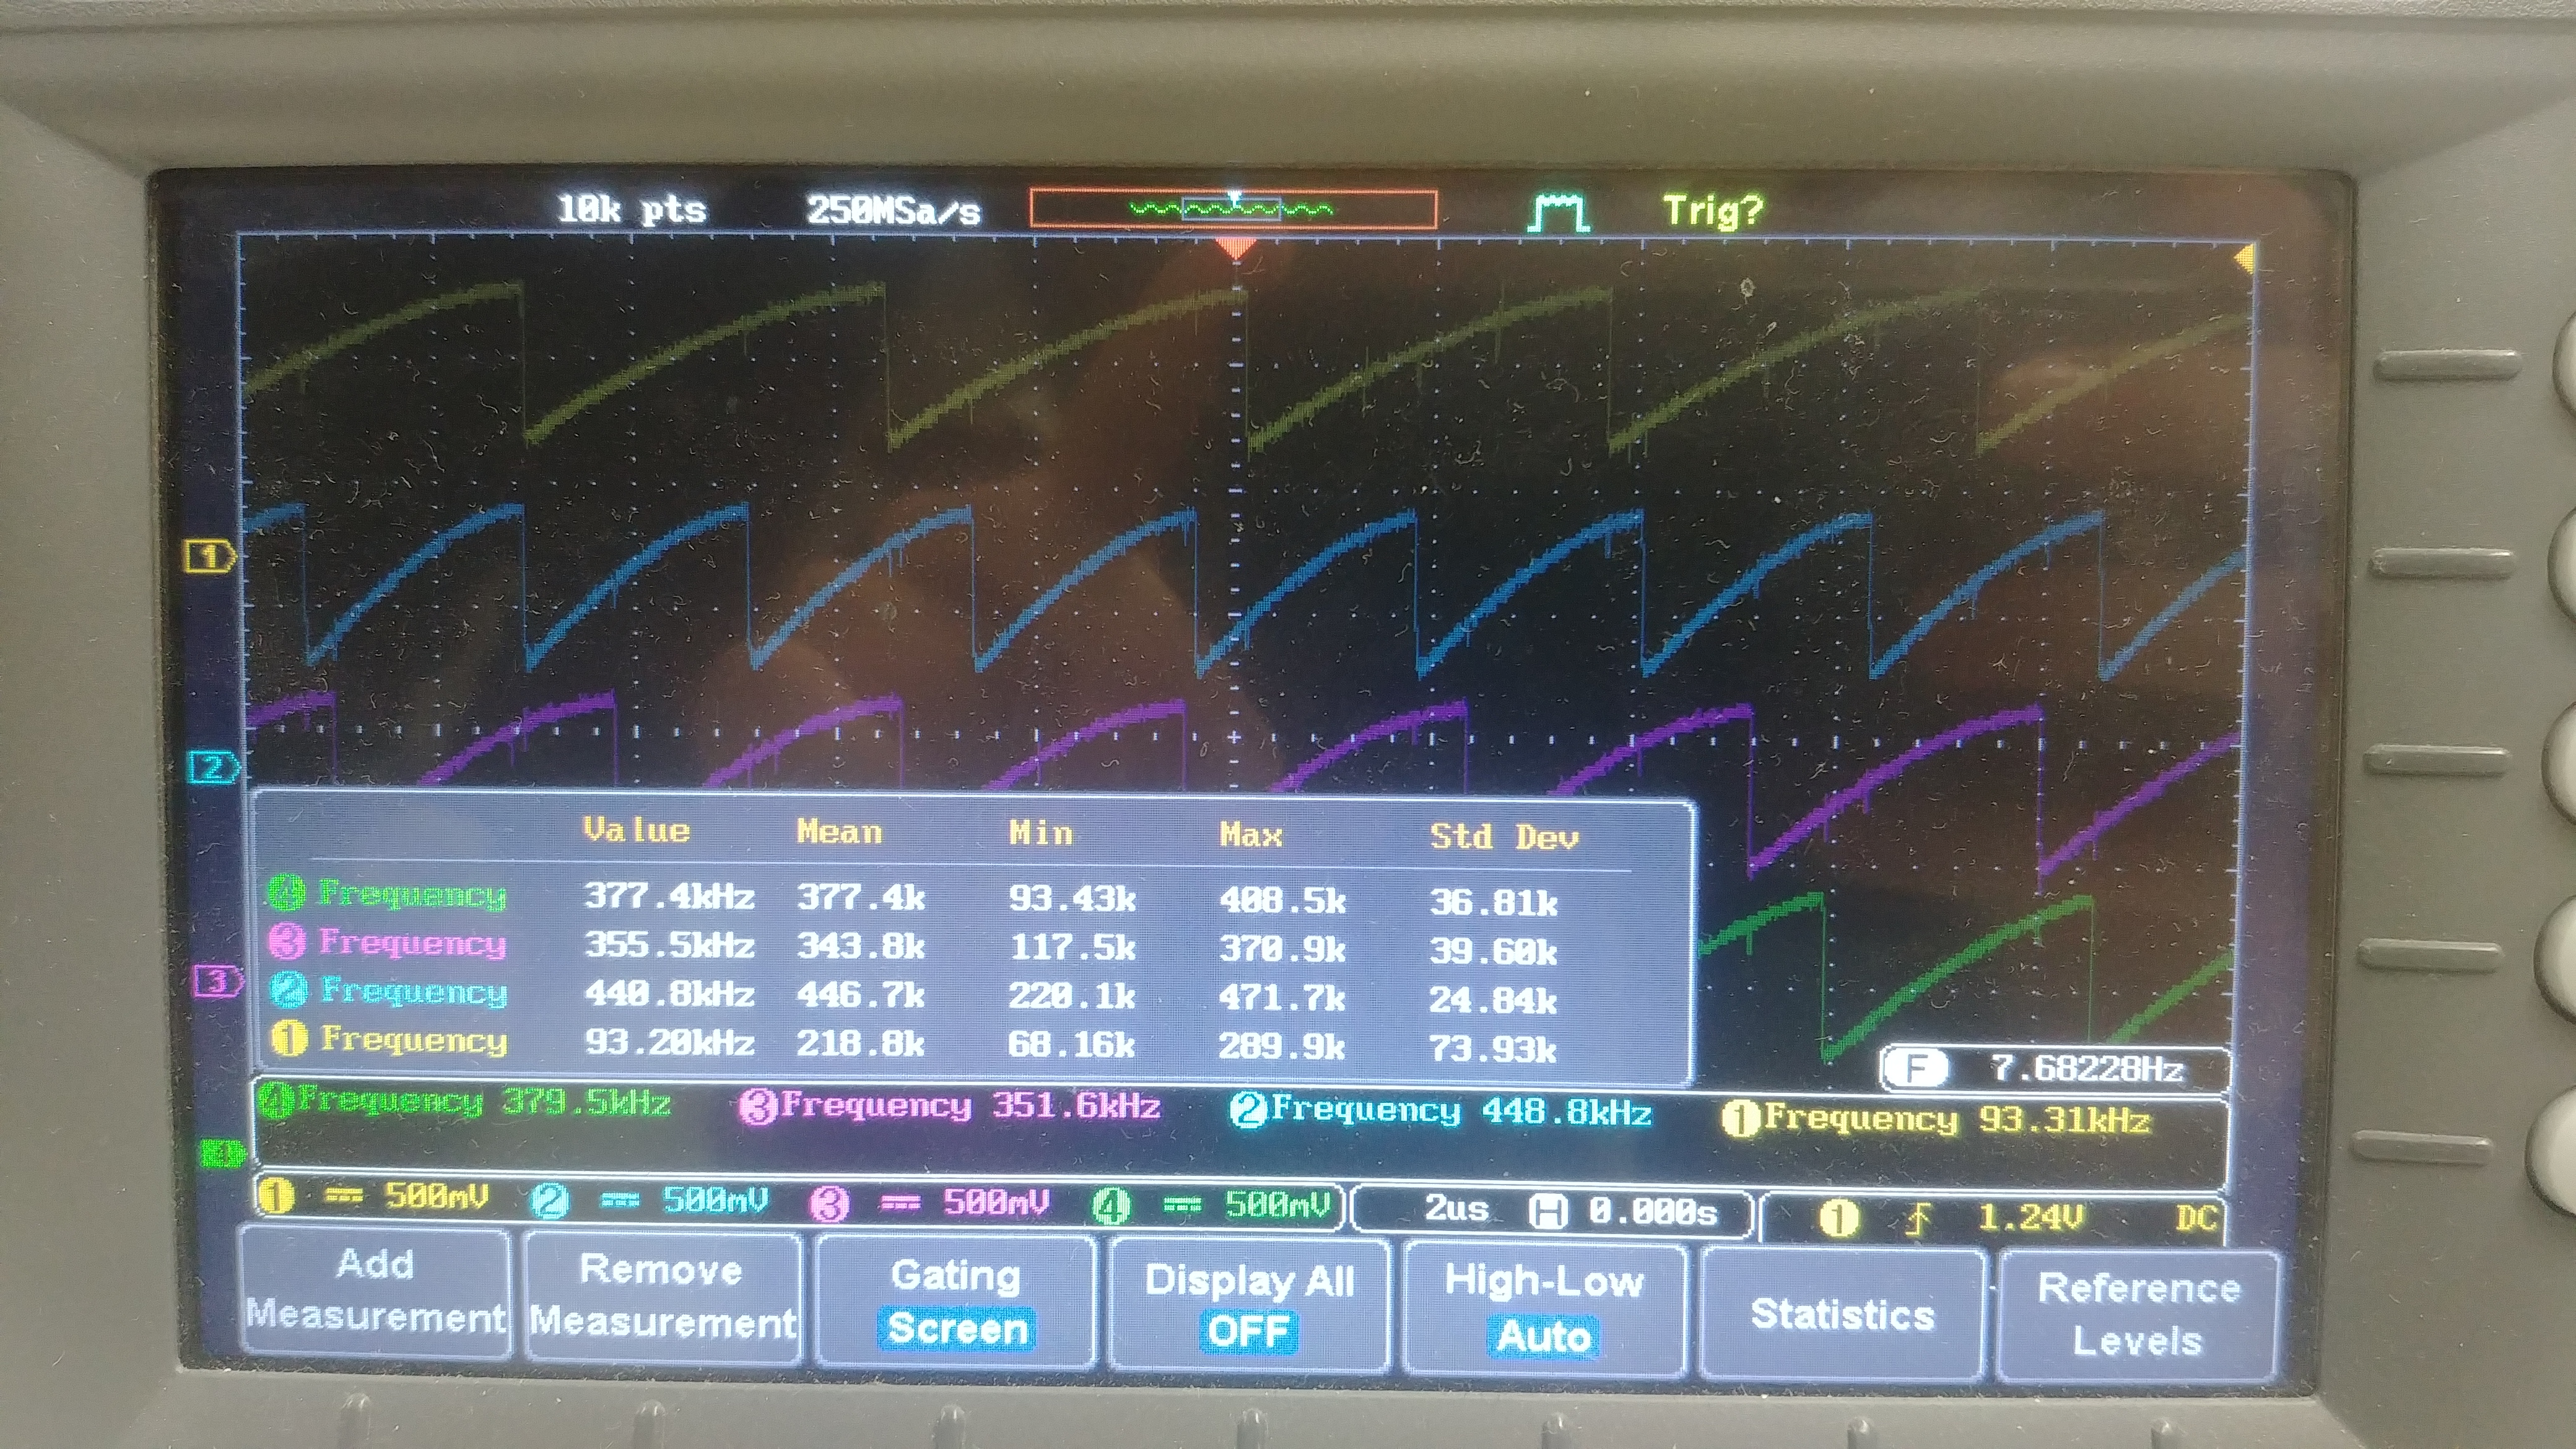
\includegraphics[scale=0.04]{pictures/oszilloskop_pic_2.jpg} 
\end{center}
\end{figure}

\begin{table}[H]
\centering
\captionsetup{justification=centering}
\caption{Feuerrate der vier Neuronen}
\begin{tabular}{l|l}
 Neuron&Feuerrate\\
\hline
$1$&$377.4 \pm 36.8$kHz\\
$2$&$343.8 \pm 39.6$kHz\\
$3$&$446.7 \pm 24.8$kHz\\
$4$&$218.8 \pm 73.9$kHz
\end{tabular}
\label{tab:01}
\end{table}

\newpage


\subsection{Aufgabe 4}
Über die Variation der Leitfähigkeiten $g_{leak}$ kann die Feuerrate verändert werden. Wir kalibrieren die 4 Neuronen für eine identische Feuerrate und damit identische Membranzeitkonstante, indem wir einen neuen Leckleitwert $g_{leak}'$ für jedes Neuron einstellen. Zur Berechnung von $g_{leak}'$ verwenden wir folgende Überlegung:
\begin{align*}
f_{firing}&=g_{leak}/C_m\\f_{firing}‘&=g_{leak}/C_m*1/g_{leak}*g_{leak}’\\&=f_{firing}/g_{leak}*g_{leak}’\\g_{leak}’&=f_{firing}‘/f_{firing}*g_{leak}
\end{align*}

\noindent Setzen wir die entsprechenden Werte ein, so erhalten wir:

\begin{table}[H]
\centering
\captionsetup{justification=centering}
\caption{Neue $g_{leak}'$ Werte der vier Neuronen}
\begin{tabular}{l|l}
 Neuron&$g_{leak}'$\\
\hline
$1$&$145.6 nS$\\
$2$&$90.8 nS$\\
$3$&$115.1 nS$\\
$4$&$107.5 nS$
\end{tabular}
\label{tab:01}
\end{table}

\noindent Die Schwankungen kommen von Herstellungsungenauigkeiten (fixed pattern noise). Zudem ist uns aufgefallen, dass es eine gewisse trial to trial Variabilität gab (durch elektrisches und thermisches Rauschen). 


\subsection{Aufgabe 5}
Wie man sehen kann, erhält man eine asymmetrische Verteilung, die Poissonartig aussieht. Dies ist in sehr guter Übereinstimmung mit dem Histrogramm aus der Versuchsanleitung.


\begin{figure} [ht]
\begin{center}
\label{fig:abb4}
\caption{Histogramm der Membranzeitkonstanten von 192 unkalibrierten Neuronen}
\includegraphics[scale=0.35]{pictures/firing_rates.pdf} 
\end{center}
\end{figure}


\newpage


\section{Einzelnes Neuron mit synaptischem Input}
In dieser Aufgabe bewerten wir den Einfluss des synaptischen Inputs auf das Neuron.


\subsection{Aufgabe 1}
Die Parameter drvifall und drviout werden variiert, dabei wird beobachtet, dass die EPSP-Kurve für kleine Werte von drvifall schneller abfällt und der Peak wird größer. Für kleinere Werte von drviout wird der Peak hingegen leicht kleiner und die EPSP-Kurve fällt minimal langsamer ab.

\begin{figure} [ht]
\begin{center}
\label{fig:abb6}
\caption{EPSP mit Parametern drvifall=1.5, drviout=1.6}
\includegraphics[scale=0.35]{pictures/epsp_fall_1_5_out_1_6.pdf} 
\end{center}
\end{figure}

\begin{figure} [ht]
\begin{center}
\label{fig:abb7}
\caption{EPSP mit Parametern drvifall=0.1, drviout=1.6}
\includegraphics[scale=0.35]{pictures/epsp_fall_0_1_out_1_6.pdf} 
\end{center}
\end{figure}

\begin{figure} [ht]
\begin{center}
\label{fig:abb8}
\caption{EPSP mit Parametern drvifall=1.5, drviout=0.3}
\includegraphics[scale=0.35]{pictures/epsp_fall_1_5_out_0_3.pdf} 
\end{center}
\end{figure}


\subsection{Aufgabe 2}
Wie erwartet ist der Peak umgekehrt. Das Verhalten der beiden Parameter drvifall und drviout ist hingegen unverändert im Vergleich zum EPSP.


\begin{figure} [ht]
\begin{center}
\label{fig:abb9}
\caption{IPSP mit Parametern drvifall=1.5, drviout=1.6}
\includegraphics[scale=0.35]{pictures/epsp_inhibitory_fall_1_5_out_1_6.pdf} 
\end{center}
\end{figure}


\subsection{Aufgabe 3}
Wir untersuchen das fixed-pattern noise zwischen verschiedenen Synapsen. Hierzu werden von 192 Synapsen gemittelte EPSP-Läufe aufgenommen und deren Höhe bestimmt. Die Verteilung ist als Histogramm in Abbildung \ref{fig:abb10} zu sehen. Die berechnete Varianz der EPSP-Höhen beträgt $\sigma^2= 23.14mV^2$.

\begin{figure} [ht]
\begin{center}
\label{fig:abb10}
\caption{Histogramm der EPSP-Höhen von 192 Synapsen}
\includegraphics[scale=0.35]{pictures/epsp_heights.pdf} 
\end{center}
\end{figure}



\subsection{Aufgabe 4}
In einem zusätzlichen Skript zu dieser Aufgabe (fp_task3_synin_epsp_stacked.py) finden Sie
kommentierte Zeilen für eine andere Stimuluserzeugung. Verwenden Sie diesen Stimulus zur Beobachtung gestapelter
EPSPs auf der Membran zu beobachten, und reduzieren Sie den zeitlichen Abstand zwischen den Eingangs-Spikes
bis das Neuron mindestens einmal feuert. Dazu darf der Schwellenwert nicht auf einen großen
Wert gesetzt werden.
Vergleichen Sie die relativen Höhen der verschiedenen PSPs qualitativ mit den vorherigen Ergebnissen des festen
Muster-Rausch-Ergebnissen. Beachten Sie, dass die Eingangs-Spikes von verschiedenen Synapsen
Treibern stammen. Berücksichtigen Sie Ihre Ergebnisse bezüglich des Rauschens mit festen Mustern: Was erwarten Sie?

Übersetzt mit www.DeepL.com/Translator (kostenlose Version)

\newpage


\section{Kurzzeit-Plastizität}


\subsection{Aufgabe 1}


\subsection{Aufgabe 2}


\subsection{Aufgabe 3}


\newpage


\section{Feed-Forward Netzwerke}
In diesem Versuchsteil wird erstmals ein neuronales Netz am Beispiel einer vorwärts gerichteten Synfire Chain untersucht. Der Aufbau erfolgt gemäß Abbildung \ref{fig:abb11100}. Die Kettenglieder sind Populationen und bestehene aus einer gewissen Anzahl Neuronen. Jede Population ist jeweils mit der nächsten Population verbunden. Eine Gruppe (Spalte) feuert dabei immer synchron. Die inhibitorischen Neuronen verhindern ein Doppelfeuern der exzitatorischen. 

\begin{figure} [ht]
\begin{center}
\label{fig:abb4}
\caption{Schematische Darstellung einer Synfire-Kette mit Feed-Forward-Hemmung. Erregende und hemmende Neuronen sind rot bzw. blau gefärbt}
\includegraphics[scale=0.35]{pictures/example.png}
\end{center}
\end{figure}

\subsection{Aufgabe 1}

\begin{figure} [ht]
\begin{center}
\label{fig:abb4}
\caption{Emuliertes Netzwerk: Aktivität der Synfire-Kette einschließlich des Membranpotenzials des Neurons mit ID=0}
\includegraphics[scale=0.35]{pictures/feed_forward_synfire_behavior.png}
\end{center}
\end{figure}

\subsection{Aufgabe 2}


\subsection{Aufgabe 3}


\newpage


\section{Rekurrente Netzwerke}


\subsection{Aufgabe 1}


\subsection{Aufgabe 2}


\subsection{Aufgabe 3}


\newpage


\section{Eine einfache Berechnung - XOR}


\subsection{Aufgabe 1}


\subsection{Aufgabe 2}


\subsection{Aufgabe 3}


\subsection{Aufgabe 4}





\end{document}
